\section{\LARGE Task one:}
\begin{IEEEkeywords}
    Config \& Kernel Development
\end{IEEEkeywords}
\vspace{-0.3cm}
\subsection{Environment config:}
\subsubsection{}~Use WSL2 to deploy Ubuntu\newline
One of the advantages of using WSL2 is The Ubuntu could \underline {connect directly the graphic card }
of ur Windows host! \newline
\newline 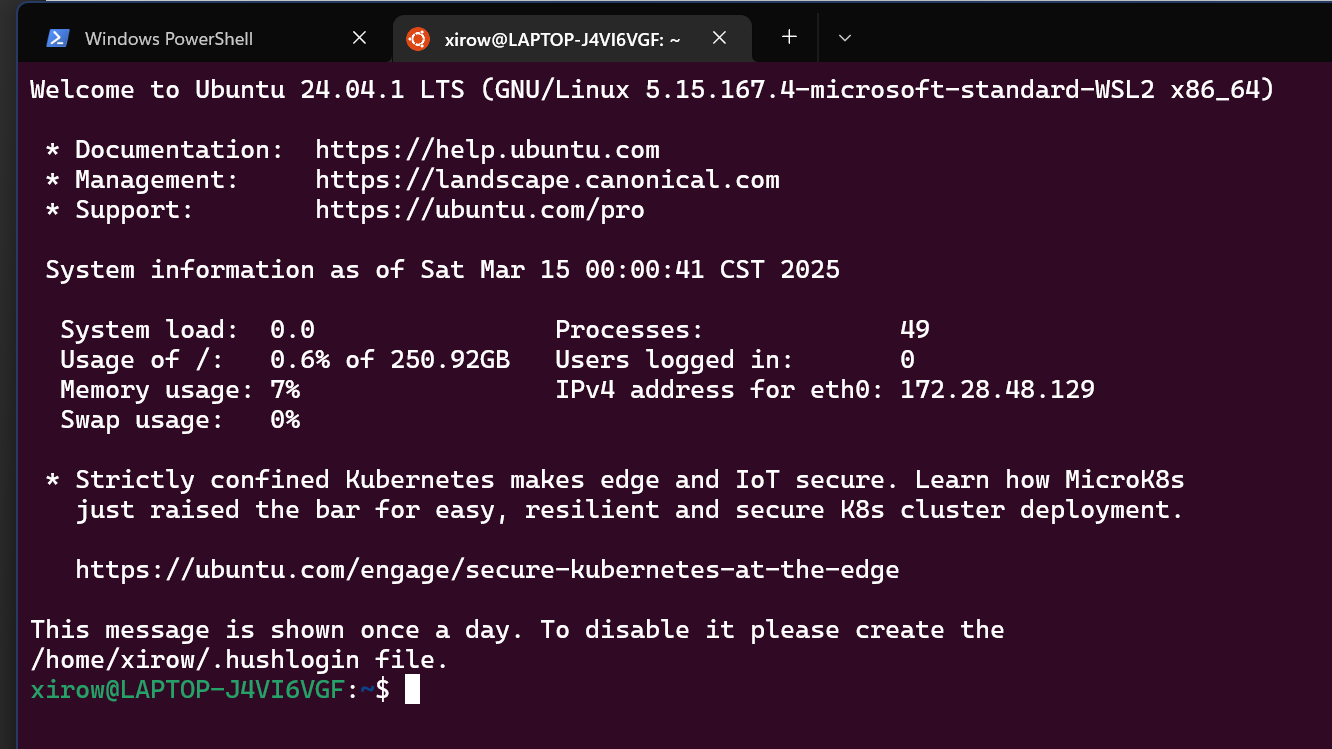
\includegraphics[width=3.3in]{photograph/ubuntu}\newline


\subsubsection{}~Deploy CUDA Toolkit and Pytorch\newline
search the method of installing CUDA and PyTorch in Ubuntu and configure the environment.\newline~
\newline Firstly, employing the CUDA:\newline
\newline 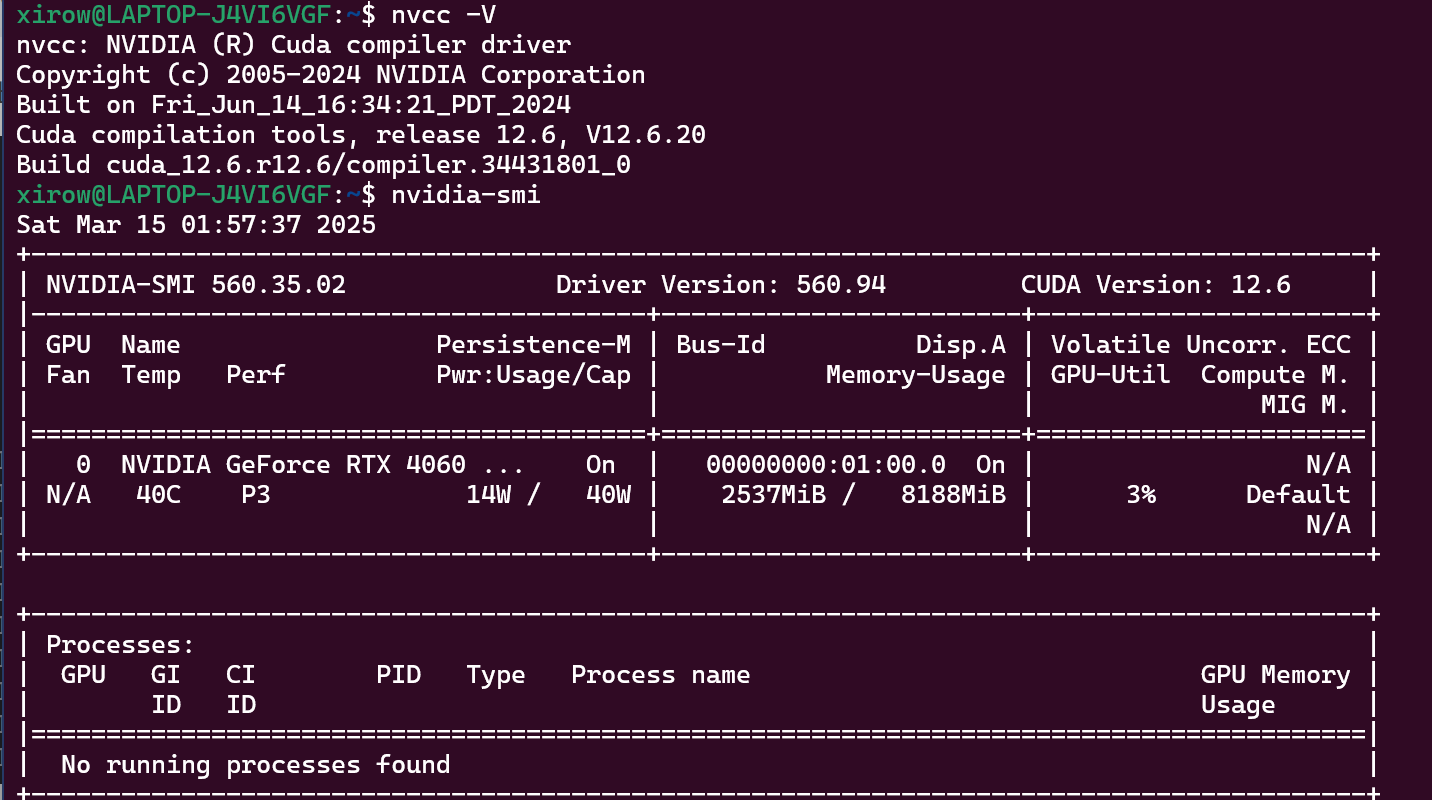
\includegraphics[width=3.3in]{photograph/cuda.png}\newline
\newline Secondly, configuring the conda environment.
I decide to use it to carry my python and pytorch environment for its advantages:
1.isolating dependencies 2.simplifying manage of dependencies
3.Supporting Cross-platform\newline
~\newline ~\newline~\newline~\newline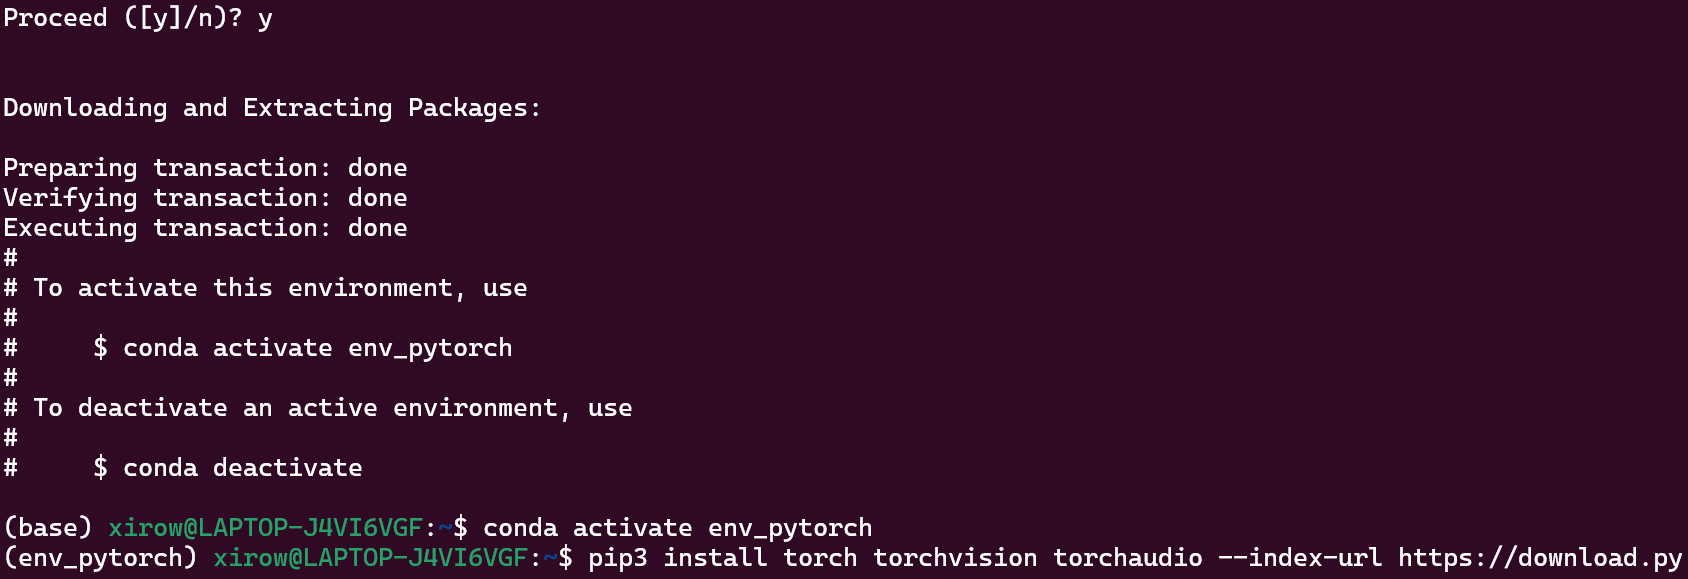
\includegraphics[width=3.3in,height=1.4in]{photograph/conda.png}\newline
\newline Then installing the PyTorch Frame:\newline
Detecting GPU and the computing of cuda!
\newline 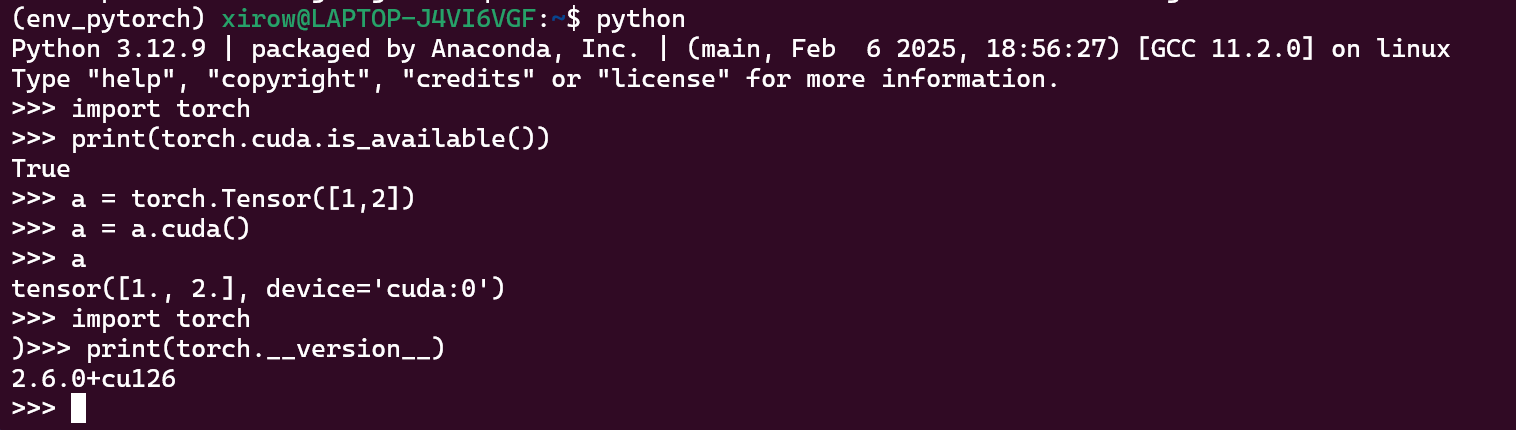
\includegraphics[width=3.3in,height=1.7in]{photograph/pytorch.png}\newline

\subsubsection{}~GPU computing power\newline
Verify the availability of the GPU computing power by using nvprof.\newline
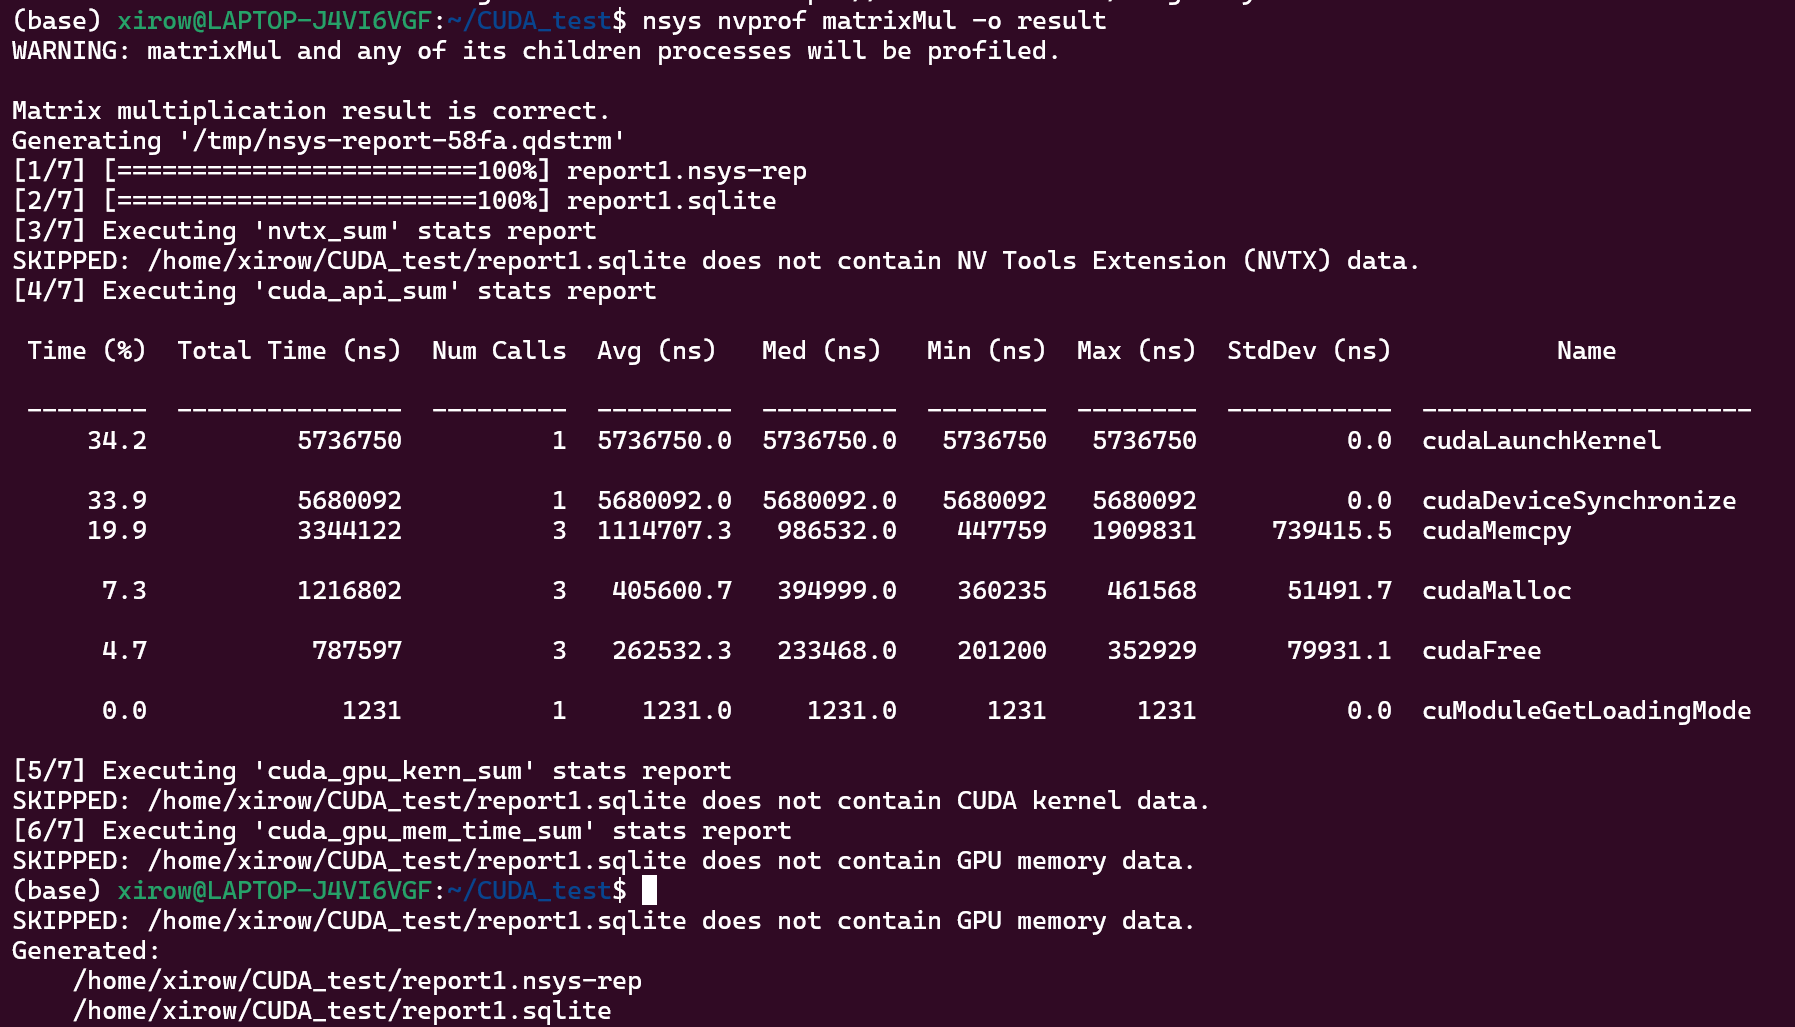
\includegraphics[width=3.3in]{photograph/nvprof.png}\newline

\subsection{Exploit CUDA kernel:}
\subsubsection{}~To pave the way for exploiting kernel\newline
\rule{\textwidth}{0pt}
\rule{\textwidth}{0pt}
Firstly\newline
CUDA program:\newline
I had a general understanding of cuda programming through study a course of it, which made me
have a moderate command of cuda, such as: kernel function,memory model of cuda,thread-block-warp,
resource allocation,error check\dots\newline
\rule{\textwidth}{0pt}
\rule{\textwidth}{0pt}
Secondly\newline
LayerNorm\newline
LayerNorm are always broken apart into two parts which is normalization and then by layers:\newline
When training for neural net,we often use LayNorm to avoid gradient disappearance or gradient explosion.
LayerNorm could encapsulate those values produced by neurons within a much small range,typically centered
around zero. What this allow for is much more \underline{stable training} as we actually perform a gradient step!\newline
And every neuron in every layer is normalized such that all the activation will have a center like zero or
standard deviation of one!\newline 
The following is the formula to achieve LayerNorm:\newline
\[
\hat{x_{i}} = \frac{x_{i} - \mu}{\sqrt{\sigma^2 + \epsilon}}
\]
$\epsilon$~~is a small value to avoid zero appearing in denominator\newline
simplifying:
\[
\hat{x_{i}} = \frac{x_{i} - \mu}{\sigma}
\]
\[
\mu = \frac{1}{n}\sum_{i=1}^nx_{i} \qquad
\sigma = \sqrt{\frac{1}{n}\sum_{i=1}^{n}(x_{i} - \mu)^2}
\]
\vspace{0.5cm}
\subsubsection{}~process of exploiting kernel\newline
\rule{\textwidth}{0pt}
\rule{\textwidth}{0pt}
Firstly\newline
Using vector float4 to access memory:\newline
Through reading four floats one times to reduce times of accessing memory so that it can improve efficiency.
It also takes advantage of the power of \underline{parallel computing} better!
\rule{\textwidth}{0pt}
\rule{\textwidth}{0pt}
Secondly\newline
Using Warp Reduce:\newline
It is such an efficient optimizing technology which can reduce the computing complexity.Because a cuda core
computes in parallel in warps which contain 32 threads.So using some instructions to make the thread execute
computing tasks simultaneously.In that case,We can apply Warp Reduce to every adding calculation!\newline
\rule{\textwidth}{0pt}
\rule{\textwidth}{0pt}
Thirdly\newline
Supporting Dynamic shapes automatic adaptation:\newline
Calculating the size of grid and block dynamically.
Parameterize the kernel using templates or macros.
Dynamic Parallelism.\newline
\rule{\textwidth}{0pt}
\rule{\textwidth}{0pt}
Fourthly\newline
Realizing Shared-memory Double Buffering system to avoid Bank Conflict:\newline
The core idea of it is using two shared memory areas,one of which is used to read another is used to write.
So that when a buffer is being used, another can load and store to improve efficiency!
\rule{\textwidth}{0pt}
\rule{\textwidth}{0pt}
{\LARGE The whole code is on my github repository!}
